\chapter{Network Design}

\section{Topology}

The topology used for this lab assignment took the form of a three router set-up, 
simulating an infrastructure a typical Internet Service Provider (ISP)
might have. Using three routers as opposed to a one allowed our ISP to make
use of technologies such as dynamic internal routing and iBGP in order to
create a fault-tolerant network. Joining our routers in a complete graph
introduced maximum redundancy and allowed for increased uptime as any traffic
could of been routed via an alternate path were an outage occur on any single
device.

\begin{figure}[!ht]
    \caption{High-level Topology}
    \centering
    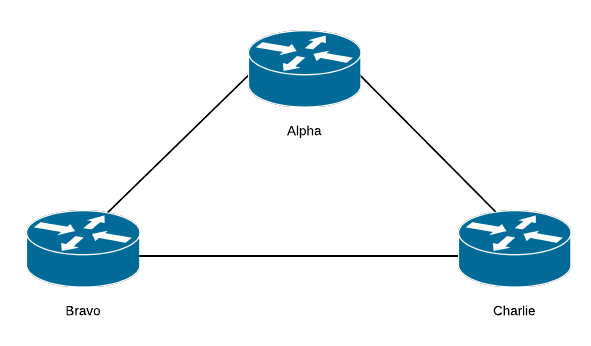
\includegraphics[width=0.8\textwidth]{images/networkTopology.png}
\end{figure}

\section{Address Allocation}
\subsection{IPv4}
For this lab exercise we were assigned the IP address space
\texttt{12.0.0.0/8}. This provided us with the ability to allocate 16.7 million
addresses, of which only a small fraction were required for our network
infrastructure. Even so, we took into account the issues that arose from the
original distribution of excessively large IPv4 network blocks to ISPs,
businesses, educational institutions, etc~\cite{ipv4alloc}\cite{internetmap}
and decided it was best to be conservative in our allocations. With this in
mind we invented three classifications of network address, each defining the
minimum subnet size deemed necessary for its purpose. These are outlined in
Figure~\ref{figure:network-alloc-1}.

\begin{figure}[!ht]
    \caption{Classifications of Network Allocations}
    \label{figure:network-alloc-1}
    \centering
    \begin{tabular}{|c|c|p{5.5cm}|}

        \hline
        \textbf{Address Type} & \textbf{Subnet Mask} & \textbf{Justification} \\

        \hline
        Customer Segment & \texttt{/24} & These were allocated to downstream
        customers, who were given enough address space for 254 devices. In our
        network, laptops were used on these segments to test connectivity to
        customers. The size of this subnet also allowed for easy identification
        of subnets to their location in the topology.\\

        \hline
        Point-to-point Links & \texttt{/30} & This was used for links that
        connected two routers, because for those links only two IP Addresses
        were required and a \texttt{/30} subnet mask is the smallest mask that
        can provide this.
        \textbf{Note:} The connection to our provider, AS 42, was an exception
        to this and used a \texttt{/24} subnet mask as was provided by AS 42.\\

        \hline
        Loopback Address & \texttt{/32} & These were addresses used for the
        loopback interfaces on the routers. There was only a requirement for a
        single address and a \texttt{/32} mask produced this.\\

        \hline
    \end{tabular}
\end{figure}
In addition to the classification of subnets based on size, we used several IP
schemas to choose the IP values of our networks from our allocated block. This
allowed for quick identification of a network from its IP without referencing
our network diagrams. For example, customer segments connected to the Alpha
router had a third octet value of 1, so it was immediately apparent that the IP
\texttt{12.0.1.0/24} was connected to Alpha.

These conventions were decided in advance of our network build-out and helped
us diagnose issues with IP or interior routing configurations in a more
intuitive way. The exact schemas are outlined in Figure~\ref{figure:network-alloc-2}.

\begin{figure}[!ht]
    \caption{IP Schemas}
    \label{figure:network-alloc-2}
    \centering
    \begin{tabular}{|p{3cm}|p{3cm}|p{5cm}|}

        \hline
        \textbf{Schema} & \textbf{Classification} & \textbf{Identifying Feature} \\

        \hline
        \texttt{12.0.\#.0/24} & Customer Segment & The hash dictates the ISP
        router that this address space would be connected to, 1 through 3 for
        Alpha, Bravo and Charlie. This could be scaled up to 253 additional
        subnets in the Service Provider.\\
        \hline
        \texttt{12.\#.0.0/30}, where $\#> 10$ & Peer Point-to-point Link &
        The hash in these networks dictates the assigned number of the group we
        connect to on these links. This enabled us to quickly identify the
        group involved with any connectivity issues using BGP. For example, the
        link to group 3 used the network \texttt{12.13.0.0/30}.\\
        \hline
        \texttt{12.0.0.\#/30} & Internal Point-to-point Link &
        The hash is a multiple of 4, starting from 0. This choice was
        arbitrary.\\
        \hline
        \texttt{12.\#.\#.\#/32} & Loopback Address & The hash is
        the same value in all three octets of the address and dictates the
        router that this loopback was assigned to. For example,
        \texttt{12.3.3.3/32} was the loopback address of Charlie.\\

        \hline
    \end{tabular}
\end{figure}

\clearpage

\subsection{IPv6}
When allocating the IPv6 address-space we took a similar approach to that of
IPv4, aiming to allocate an appropriate sized address block to each segment of
the network. As such the classifications used are approximately the same as
IPv4, with network segments being either a Customer Segment, Point-to-point
link or a Loopback. This is detailed in Figure~\ref{figure:network-alloc-3}.

\begin{figure}[!ht]
    \caption{Classifications of Network Allocations}
    \label{figure:network-alloc-3}
    \centering
    \begin{tabular}{|c|c|p{5.5cm}|}

        \hline \textbf{Address Type} & \textbf{Subnet Mask} & \textbf{Justification} \\

        \hline
        Customer Segment & \texttt{/36} & This address space was allocated for
        downstream connections to the ISPs customers. It had a large subnet
        mask to allow for it to be broken down into subnets containing the
        48-bit Global Routing Prefix for customer networks.\\

        \hline
        Point-to-point Links & \texttt{/64} & These addresses were used for
        links that directly connected two routers, requiring two unique IP
        addresses. Reasons for the size of the subnet mask used are discussed
        below.\\

        \hline
        Loopback Address & \texttt{/128} & Addresses used for the loopback
        interfaces on the routers, there was only a requirement for a single
        address as was the case with IPv4. In IPv6 a \texttt{/128} mask
        produces this.\\

        \hline
    \end{tabular}
\end{figure}

Customer Segments used a \texttt{/36} mask as a method of breaking down our
customer networks into a more manageable block of addresses. The \texttt{/36}
mask allowed for us to further break down our Customer Segments into IPv6
blocks with a 48-bit Global Routing Prefix, which is a unique ID for an IPv6
address which can be used identify both the ISP and the customer.

In Figure~\ref{figure:network-alloc-3} it is obvious that applying a
\texttt{/64} mask allocates a considerable amount of addresses to a network
which would otherwise only require two unique addresses. The decision to use
this address was taken from RFC 4291, which dictates that ``For all unicast
addresses, except those that start with the binary value 000, Interface IDs are
required to be 64 bits long''~\cite{rfc4291}. In recent years there have been
discussions that the allocation of such a large amount of addresses is wasteful
and that the use of a \texttt{/127} mask should be endorsed. However this is
not a standard and for the purposes of this lab we have adhered to the RFC instead.
